% !TEX root = ../main.tex

\chapter{方法}

\section{研究定位与总体设计思路}
手势可根据语义依赖性与时间结构复杂度区分为可语义生成与可韵律生成两大类。
本文的研究聚焦于严格实时的语音驱动任务,在此条件下模型无法访问未来语音或完整语义,
因此重点生成与语音韵律同步的 \emph{beat-like} 手势及头部动作,
并通过面部与头部模态的联合输入进一步增强表达性与自然度。
这种选择既符合认知语言学的节奏—动作一致性原则,也符合实时系统的因果约束。

基于上述定位,本文提出了一种基于音频、面部 BlendShape 权重和头部姿态输入的
帧级多模态级联手势生成模型 \emph{FaceCapGes}。
模型旨在在实时条件下实现自然、同步且具有一定指向性的上肢动作生成,
在不依赖语义理解或未来上下文的前提下,
通过多模态输入弥补语音模态预测能力的不足。
整体架构包括三个阶段:
(1)模态编码;(2)躯干与手部动作生成(基于 LSTM 与 MLP);(3)对抗优化模块。
各部分结构将在后续小节中详细介绍。

\section{系统整体框架与模块定位}

为实现基于语音、面部捕捉与头部姿态的实时数字人驱动系统,本文首先构建了完整的信号采集、动作生成与渲染展示的处理管线。FaceCapGes 模型作为该系统的核心计算模块,负责在实时约束下从多模态输入推理出当前帧的上半身骨骼姿态。整个系统框架如图~\ref{fig:overallFramework} 所示。

\begin{figure*}[h!t]
\centering
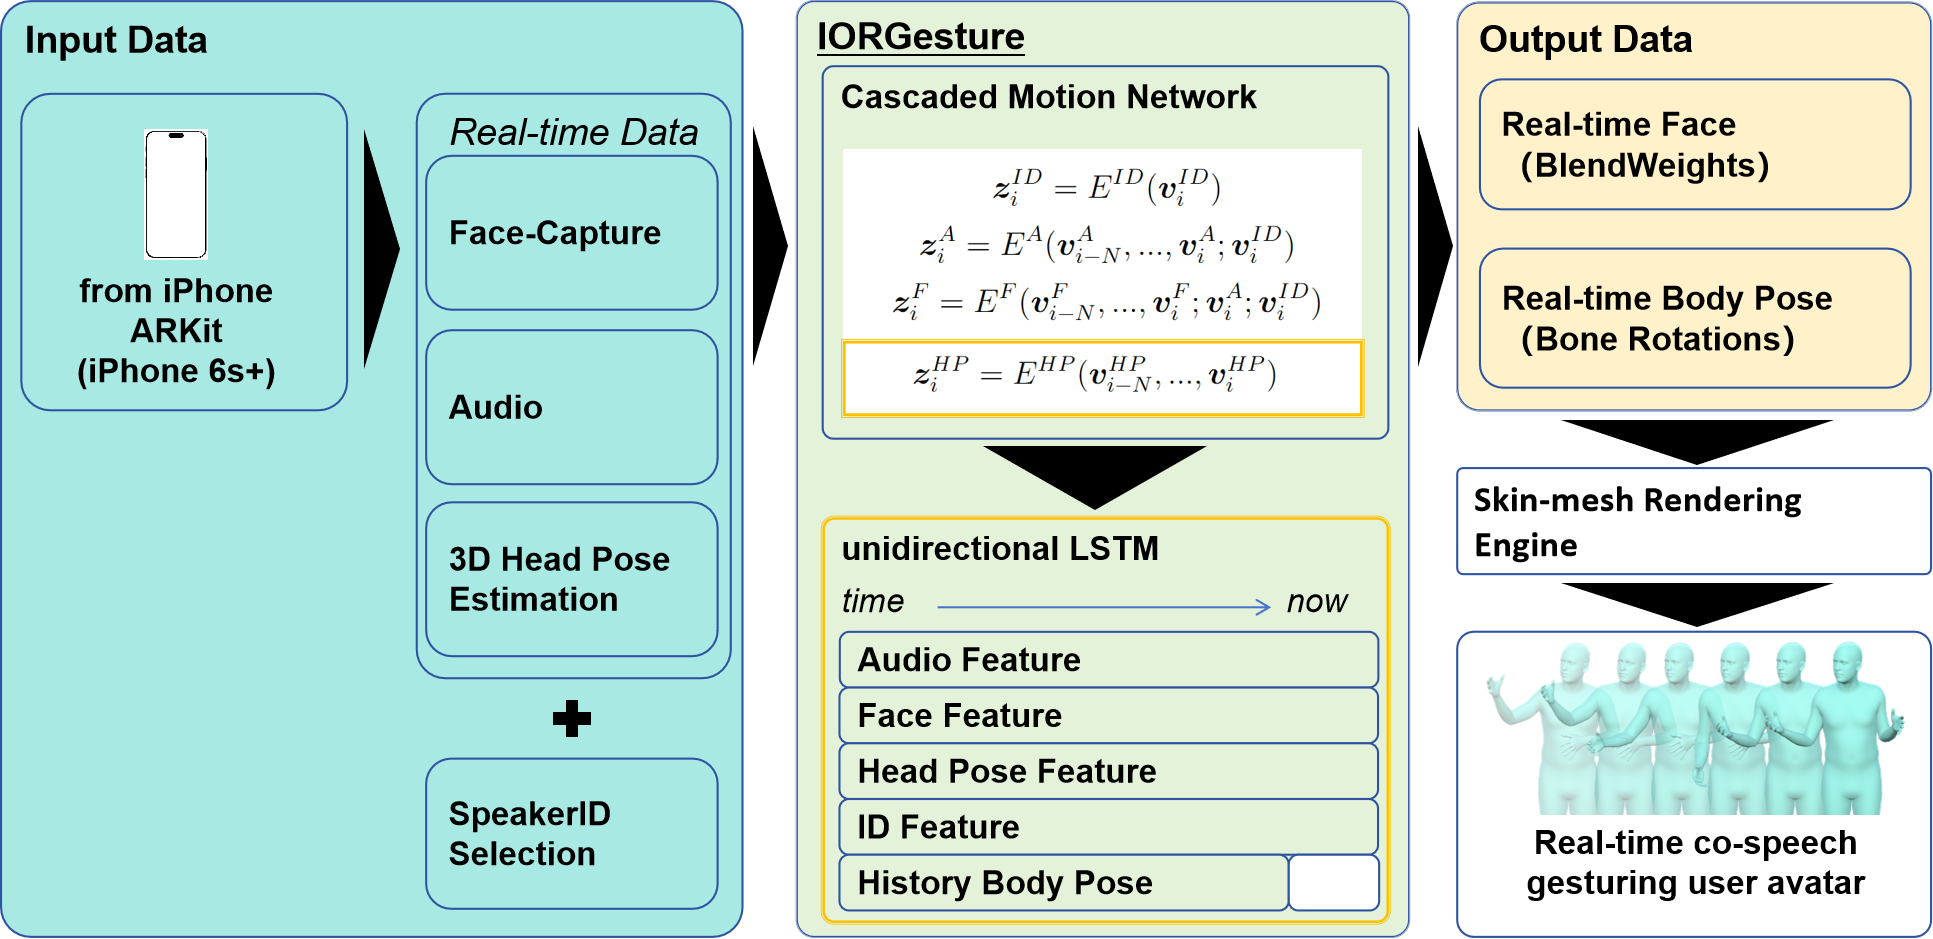
\includegraphics[width=\textwidth]{figures/FigOverallFramework.png}
\caption{系统整体框架与数据流示意图}
\label{fig:overallFramework}
\end{figure*}

\paragraph{说话人配置选择.}
图~\ref{fig:overallFramework} 中的 “Speaker ID Selection” 模块仅用于系统层的模型切换,
而非模型输入的一部分。
在部署时,FaceCapGes 针对每位演讲者独立训练一组参数,
用户选择说话人 ID 时,系统仅加载对应权重文件,
相当于切换“说话风格配置文件”。
因此,网络内部不读取 ID 向量,也不会在推理过程中动态更换风格,
从而保持实时性与运行稳定性。

\paragraph{面部模态的外部传递.}
FaceCapGes 的输出仅包含上半身骨骼姿态,
面部 blendshape 系数则由独立的实时面部捕捉模块生成,
并直接传入虚拟人渲染引擎。
模型输入端读取这些 blendshape 作为语义线索,
但不对其进行预测或重建。
表情捕捉与动作生成在信号层面独立运行。

系统整体可分为三个主要模块:输入采集模块、实时手势生成模块与渲染驱动模块。
其中,FaceCapGes 对应于实时手势生成部分,是整个管线的核心计算组件。

\subsection{输入采集模块}

该模块负责从用户端设备实时获取多模态输入信号,包括图像流与音频流两部分。

图像输入:前置 RGB 摄像头采集用户面部视频流,并交由 Apple ARKit 模块进行面部追踪与表情解析。ARKit 输出两类信息:

面部 BlendShape 权重向量(共 52 维),描述面部肌肉的形变状态,用于反映用户的情绪与口型变化;

头部姿态参数,以三维旋转形式(yaw、pitch、roll 或对应旋转矩阵)表示头部的朝向与转动幅度。

音频输入:系统通过麦克风实时采样用户语音信号。音频流经特征提取模块(如 Mel 频谱、短时能量、基频 F0 等),得到高维时间序列向量,为后续的语音节奏分析提供基础特征。

以上三类信号——音频、面部 BlendShape、头部姿态——均以帧为时间单位同步采集。系统在采样阶段保持统一时间戳,以保证后续多模态融合时的时序对齐。

\subsection{实时手势生成模块(FaceCapGes)}

FaceCapGes 模块位于整个系统的中间层,是本文提出的关键研究部分。该模块接收来自输入采集模块的三种同步模态特征:语音特征、面部 BlendShape 权重及头部姿态参数,并在不依赖未来帧的条件下,逐帧预测用户当前时刻的上半身骨骼姿态。

生成的骨骼姿态采用 Rot6d 连续旋转表示形式,包含躯干及双臂共 47 个关节的旋转参数。
该模块通过级联多模态编码器提取特征,并利用 LSTM 解码器完成时间依赖建模,从而在保持实时性的同时,生成与语音节奏、表情变化和头部朝向高度一致的自然手势。

由于模型仅依赖当前与历史帧输入,因此可以与输入捕捉模块以固定帧率并行运行,实现端到端的低延迟推理。其平均推理时延小于 7 毫秒。

\subsection{渲染与驱动模块}

模型输出的骨骼姿态数据与面部 BlendShape 参数共同作为虚拟人驱动信号输入渲染引擎(如 Unity 或 Unreal Engine)。在引擎中,姿态参数通过骨骼绑定系统驱动上半身动作,BlendShape 参数同步驱动面部表情。渲染模块采用基于 GPU 的蒙皮计算与光照模型,以保证虚拟人动画的平滑性与实时可视化效果。

最终,系统将用户的语音、表情与身体动作以数字人的形式在屏幕或虚拟现实设备中呈现,实现低成本、无穿戴设备的实时交流体验。

综上所述,FaceCapGes 模块在整个系统中承担了“从多模态输入到上肢手势输出”的核心功能。它有效地连接了输入捕捉与虚拟人渲染环节,是实现实时数字人驱动的关键环节。下一节将正式定义该问题的数学形式,并详细介绍模型的结构设计与算法原理。

\section{问题定义}

在整体系统中,FaceCapGes 模块承担着从多模态输入信号到上肢骨骼姿态预测的核心任务。为了明确模型的输入输出结构与学习目标,本节对该问题进行形式化定义。

\subsection{任务描述}

目标是在实时条件下,根据用户当前时刻的语音、面部表情与头部姿态信息,预测其对应的上半身骨骼姿态。模型需能够逐帧生成与语音节奏、面部动态和头部转动方向相协调的自然手势动作,而不依赖未来的输入帧或整句语音信息。

形式上,可以将该任务定义为一个多模态时序映射函数:
\begin{equation}
\hat{\mathbf{B}}_t = f_\theta(\mathbf{A}_{t-N:t}, \mathbf{F}_{t-N:t}, \mathbf{H}_{t-N:t}),
\end{equation}
其中 $f_\theta$ 表示由参数 $\theta$ 控制的预测模型,$N$ 为历史窗口长度。模型仅利用当前及过去 $N$ 帧的输入信息,对当前帧 $t$ 的上半身姿态 $\hat{\mathbf{B}}_t$ 进行估计,从而满足严格的实时推理约束。

\subsection{输入与输出模态}

FaceCapGes 模型的输入由三种可同时实时获取的模态组成:语音特征、面部 BlendShape 权重及头部姿态参数;输出为当前帧的上半身骨骼旋转状态。各模态的符号与维度如表~\ref{tab:modalities} 所示。

\begin{table}[h]
\centering
\caption{输入输出模态符号与维度}
\label{tab:modalities}
\begin{tabular}{llll}
\toprule
\textbf{模态} & \textbf{符号} & \textbf{维度} & \textbf{描述} \\
\midrule
语音特征 & $\mathbf{A}_t$ & $\mathbb{R}^{1067}$ & 由音频信号提取的时序特征(Mel 频谱、能量、基频等) \\
面部 BlendShape & $\mathbf{F}_t$ & $\mathbb{R}^{52}$ & ARKit 输出的标准化表情权重向量 \\
头部姿态 & $\mathbf{H}_t$ & $\mathbb{R}^{6}$ & 采用 Rot6d 表示的头部旋转参数 \\
上半身骨骼姿态(输出) & $\mathbf{B}_t$ & $\mathbb{R}^{6 \times 47}$ & 躯干与双臂 47 个关节的旋转状态 \\
\bottomrule
\end{tabular}
\end{table}

输入序列 $(\mathbf{A}_{t-N:t}, \mathbf{F}_{t-N:t}, \mathbf{H}_{t-N:t})$ 描述了用户在过去 $N$ 帧内的语音与表情动态信息。模型通过学习其时序变化规律,逐帧生成对应的骨骼姿态输出 $\hat{\mathbf{B}}_t$。在推理阶段,模型仅访问至时刻 $t$ 的输入序列,无法访问任何未来帧信息,保证了生成过程的因果性与实时性。

\subsection{学习目标与优化形式}

在训练阶段,给定来自多模态语音动作数据集(如 BEAT)的配对样本:
\begin{equation}
(\mathbf{A}_t, \mathbf{F}_t, \mathbf{H}_t, \mathbf{B}_t),
\end{equation}
模型的学习目标是最小化预测姿态 $\hat{\mathbf{B}}_t$ 与真实姿态 $\mathbf{B}_t$ 之间的差异。
综合考虑空间重构误差与时序平滑性约束,总体优化目标可表示为:
\begin{equation}
\mathcal{L}_{total} =
\mathcal{L}_{rec} + \lambda_v \mathcal{L}_{vel} + \lambda_a \mathcal{L}_{acc} + \lambda_{adv} \mathcal{L}_{adv},
\end{equation}
其中:
\begin{itemize}
    \item $\mathcal{L}_{rec}$ 为姿态重构损失,衡量单帧旋转角度误差;
    \item $\mathcal{L}_{vel}$、$\mathcal{L}_{acc}$ 分别约束预测序列的速度与加速度连续性;
    \item $\mathcal{L}_{adv}$ 为对抗损失,用于提升生成手势的自然性;
    \item $\lambda_v, \lambda_a, \lambda_{adv}$ 为对应的权重系数。
\end{itemize}

通过最小化上述综合损失,模型能够在不依赖未来帧的条件下生成自然、流畅且与语音节奏相匹配的上肢动作序列。

\section{级联架构与输入模态设计}
\label{sec:input_encoding}

\subsection{级联架构的原理与理论背景}

现有语音驱动手势生成模型多采用多模态融合结构,其中以 CaMN~\cite{liu2022beat} 为代表的级联(cascaded)架构在语义一致性与动作自然性方面表现突出。其核心思想是将语音、面部表情与身体动作视为语义表达的不同层级:语音模态承担语义与节奏驱动作用,面部模态反映情感与意图,身体动作则是语言与情绪的外化呈现。因此,CaMN 采用自上而下的信息流:\textbf{语音 $\rightarrow$ 面部 $\rightarrow$ 动作},通过层次化结构保持模态间的语义依存关系。

这种设计符合人类交流中“语言—表情—动作”一体化的认知规律~\cite{mcneill1992hand,kendon2004gesture}。语音先规划语义与节奏,面部表情作为情绪强化信号随后产生,最终通过身体动作完成完整的非语言表达。模型中,语音编码器输出的时间嵌入被输入至面部编码器,再与面部特征融合后驱动动作解码器,从而保持语义一致性并增强表现力。

然而,CaMN 的原始设计面向离线整句生成任务,需要访问未来上下文以维持全局连贯性。在实时场景下,这种依赖将引入显著延迟并破坏因果性。FaceCapGes 在继承其层次思想的同时,对输入模式、训练方式与模态选择进行了系统性重构,以满足帧级实时约束。

\subsection{基线模态继承与实时适配}
FaceCapGes 保留了 CaMN 的语音与面部模态结构,但针对实时生成任务进行了适配性改写。

\subsubsection{说话人 ID 分支移除.}
如图 3.1 所示,系统层保留了 ‘Speaker ID Selection’ 模块用于模型切换,但该模块不属于网络输入。
在基线模型 CaMN 中,输入模态包含显式的说话人 ID 向量,用于在同一模型内区分不同演讲者的风格差异。
然而在实时交互场景下,该分支并非必要:用户身份通常固定,且说话风格的变化频率远低于帧级推理速度。
因此,FaceCapGes 移除了 ID 输入分支,并采用“单说话人训练”策略,即针对每个说话人独立训练模型参数。
实验表明,该方式能在保持收敛稳定的同时显著提升动作的自然性与节奏一致性。
从系统使用角度看,不同模型可视为“说话风格配置文件”,用户在需要时仅需切换对应参数即可,
此操作成本极低,且不影响实时性能。

\subsubsection{输入模态继承.}

语音特征通过时间卷积网络(Temporal Convolutional Network, TCN)和多层感知机(MLP)编码,以捕捉短时节奏模式;面部模态采用相似结构,并在中间层融合语音嵌入,从而增强语音与表情之间的语义关联。  
语音编码器 $E_A$ 与面部编码器 $E_F$ 的输出定义为:
\begin{equation}
\mathbf{z}^A_t = E_A(\mathbf{A}_{t-N:t}), \quad
\mathbf{z}^F_t = E_F(\mathbf{F}_{t-N:t}; \mathbf{z}^A_t),
\end{equation}
其中 $\mathbf{z}^A_t \in \mathbb{R}^{128}$,$\mathbf{z}^F_t \in \mathbb{R}^{32}$。  
这两个编码器负责提取低层次语音节奏与表情动态信息,为后续模态融合提供稳定上下文表征。

\subsubsection{输出模态继承(身体姿态解码).}

在输出端,FaceCapGes 沿用了 CaMN 的身体姿态解码模块,
用于将融合后的多模态特征映射为上半身骨骼姿态。
该部分未作结构性改动,其核心任务是将语音与面部模态编码结果与历史姿态信息结合,
生成当前时刻的躯干与手部运动。

具体而言,来自语音与面部编码器的特征
$\bm{z}_i^A$、$\bm{z}_i^F$ 会与历史姿态序列拼接,组成多模态隐向量 $\bm{z}_i^M$:
\begin{equation}
\bm{z}_i^M = \bm{z}_i^A \otimes \bm{z}_i^F \otimes (\bm{v}_{i-N}^{B}, ..., \bm{v}_i^{B}) \otimes (\bm{v}_{i-N}^{H}, ..., \bm{v}_i^{H}),
\end{equation}
其中 $\otimes$ 表示通道维度拼接操作,末帧采用零填充以对齐时间维度。
随后,$\{\bm{z}_0^M, ..., \bm{z}_N^M\}$ 经两个单向 LSTM 解码器生成躯干与手部的潜在特征:
\begin{equation}
\bm{z}^B = LSTM_B(\bm{z}_0^M, ..., \bm{z}_N^M), \quad
\bm{z}^H = LSTM_H(\bm{z}_0^M, ..., \bm{z}_N^M; \bm{z}^B),
\end{equation}
并通过独立的 MLP 模块还原为骨骼旋转向量:
\begin{equation}
\hat{\bm{v}}^B = MLP_B(\bm{z}^B), \quad \hat{\bm{v}}^H = MLP_H(\bm{z}^H),
\end{equation}
最终拼接为完整的身体姿态:
\begin{equation}
\hat{\bm{v}}^{BH} = \hat{\bm{v}}^B \otimes \hat{\bm{v}}^H.
\end{equation}

在推理阶段,解码器隐状态在时间步之间保持连续,
与前述输入模态特征配合,使模型在保持因果性的同时具备自然的时间平滑性。
由于该部分结构沿用自基线模型,本文不再赘述。
接下来,将介绍时间建模结构的改动及其对实时性的适配。

\subsubsection{时间建模结构改动与因果性约束.}

基线模型 CaMN 使用双向 LSTM(Bi-LSTM)生成完整序列的骨骼姿态,输入与输出片段长度一致。
由于双向结构在每个时间步都依赖未来帧隐状态,虽然能增强整体平滑性,但不满足实时生成场景的因果约束。
为实现严格的实时性,本文将时间建模模块改为单向 LSTM(Uni-LSTM),
使模型在每一时间步仅依赖过去 $N$ 帧的输入并预测当前帧的骨骼姿态。
虽然 Uni-LSTM 结构上仍会输出与输入片段等长的时间序列,但训练时仅计算其\textbf{最后一帧的预测误差}:

\begin{equation}
\hat{\bm{v}}_{t} = \mathrm{LSTM}(\bm{x}_{t-N:t})[-1],
\quad
\mathcal{L}_{\text{causal}} = \|\hat{\bm{v}}_t - \bm{v}_t\|_2^2.
\end{equation}

该策略使模型在前 $N$ 帧累积隐状态,于第 $N+1$ 帧完成预测,形成严格的“历史 $\rightarrow$ 当前”单向映射。

在推理阶段,FaceCapGes 采用长度为 $N$ 的显式输入窗口,并在时间步之间保留 LSTM 的隐状态。
虽然单向 LSTM 理论上能够仅通过递推隐状态存储历史信息,
但由于隐状态为压缩形式,难以完全保留短时节奏与相位特征。
因此,显式窗口输入与隐状态记忆在模型中形成互补:
前者提供局部的高分辨率上下文,
后者维持全局的时序连贯性。
这种设计在保证因果性的前提下提高了生成的稳定性与自然性,
也是实现实时语音驱动动作生成的关键因素之一。

图~\ref{fig_lstmcompare} 展示了双向与单向结构的差异:单向结构仅依赖历史帧输入,可在流式序列中逐帧输出预测结果,有效消除未来信息依赖并实现低延迟推理。

\begin{figure}[h!t]
\centering
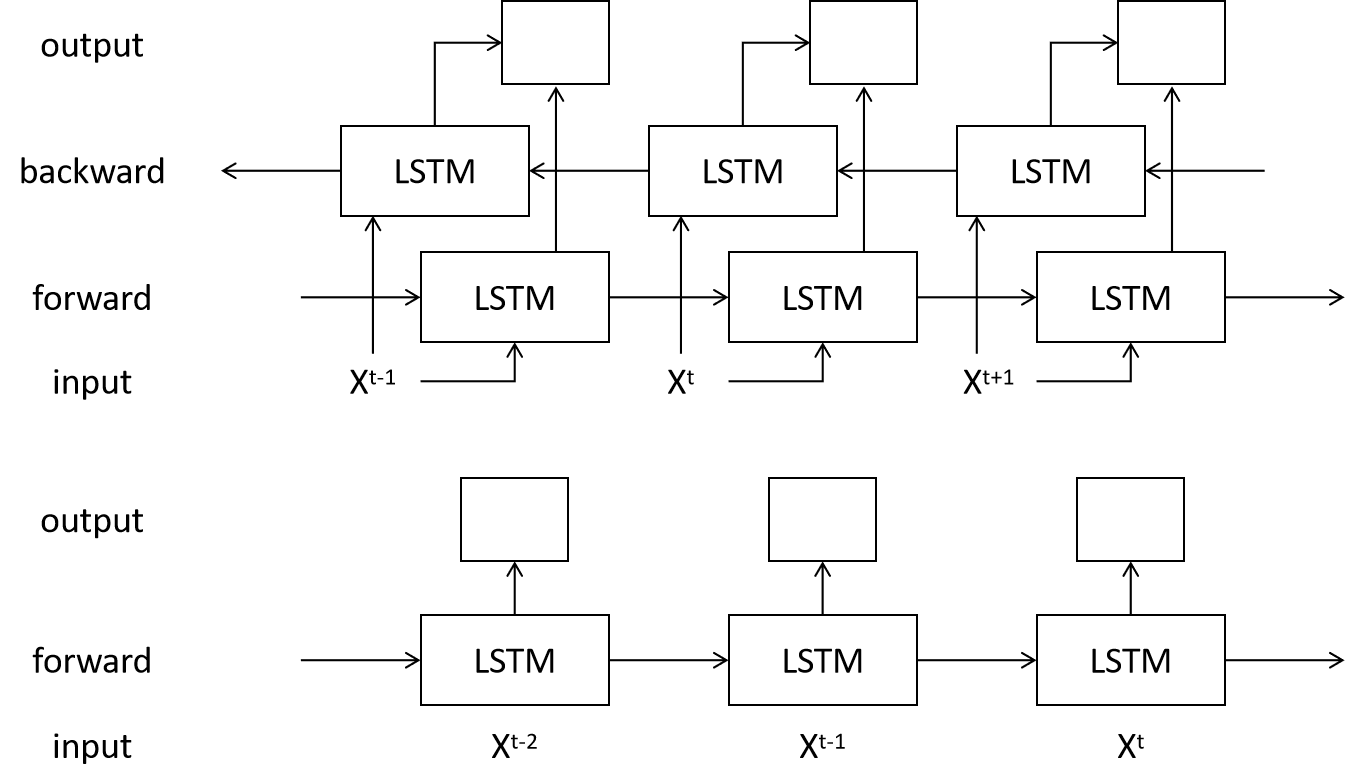
\includegraphics[width=0.9\linewidth]{figures/Fig_lstmcompare.png}
\caption{双向与单向 LSTM 对比示意图。
双向结构(上)在每一时刻依赖未来帧,需整段输入;
单向结构(下)仅依赖历史帧,可逐步生成当前姿态。}
\label{fig_lstmcompare}
\end{figure}

\subsubsection{滑动窗口式自回归训练.}

训练时,每段输入为 $N+M$ 帧,前 $N$ 帧作为输入上下文,后 $M$ 帧逐步预测(见图~\ref{fig2_})。
其中,前 $N$ 帧的历史姿态可视为模型的因果历史窗口,
其设计思路与基线模型中附加片段首部的“历史缓冲”类似,
但在意义上有所不同。
CaMN 在双向时间建模下使用该缓冲以补足片段外部上下文,
而 FaceCapGes 则将其重新定义为实时预测所需的前序姿态帧数量,
即当前帧推理所依赖的显式时间上下文。

在训练阶段,模型采用纯自回归(pure autoregressive)方式展开,
即在每一步预测后,将自身生成的历史帧作为下一步输入,
而非采用教师强制(teacher forcing)。
这种方式使模型在优化过程中暴露于自身预测的分布,
保持训练与推理过程的一致性,
避免了教师强制常见的暴露偏差(exposure bias),
即推理阶段模型面对自身生成数据时性能下降的问题。
在每个窗口内连续预测 $M$ 步后,
累计所有预测帧的误差并计算平均损失:
\begin{equation}
\mathcal{L}_{\text{total}} = \frac{1}{M}\sum_{i=1}^{M} \|\hat{\bm{g}}_i - \bm{g}_i\|_2^2.
\end{equation}

虽然该纯自回归方式在训练早期的收敛速度略慢,
但生成稳定性更高,可有效抑制长期序列中的误差积累(error accumulation)。
此外,这种机制特别契合\textbf{实时虚拟人等持续交互场景}:
模型在此类应用中并非针对短语段离线生成,
而是与语音流持续同步、长时间运行。
在这种场景下,纯自回归训练使模型在遇到自身预测误差时能够动态修正节奏,
从而在长时间交互中保持自然的动作连续性与节奏稳定性。

每一预测步中定义一个长度为 $N+1$ 的滑动窗口,
其中前 $N$ 帧为输入,第 $N+1$ 帧为预测目标。
形式化定义如下:
\begin{align}
\bm{g}^H_i &= (\bm{g}_{i-N}, ..., \bm{g}_{\min(N, i-1)}) \otimes (\hat{\bm{g}}_{\max(N+1, i-N)}, ..., \hat{\bm{g}}_{i-1}), \\
\hat{\bm{g}}_i &= FaceCapGes(\bm{v}_{i-N}, ..., \bm{v}_i; \bm{g}^H_i),
\end{align}
其中 $\otimes$ 表示时间拼接操作。
该机制在每步仅依赖过去信息,从而保持因果性约束;
同时通过窗口内的滚动更新,在不引入未来帧的前提下实现平滑过渡。
推理阶段模型以单帧为输入流,输出当前时刻的上半身姿态,实现端到端低延迟生成。

需要指出的是,由于滑动窗口机制依赖前 $N$ 帧的上下文信息,
模型在序列开端无法立即生成动作,即存在一个短暂的“冷启动”阶段。
然而在本文的目标应用场景——实时语音驱动虚拟人系统——中,
模型作为常驻进程持续运行,而非针对离散语句反复初始化。
因此该延迟仅在首次启动时出现约 $N$ 帧($0.3$--$0.5$ 秒)的等待,
对用户体验影响可忽略。
这一延迟被视为实时生成框架下的合理权衡。

\begin{figure}[h!t]
\centering
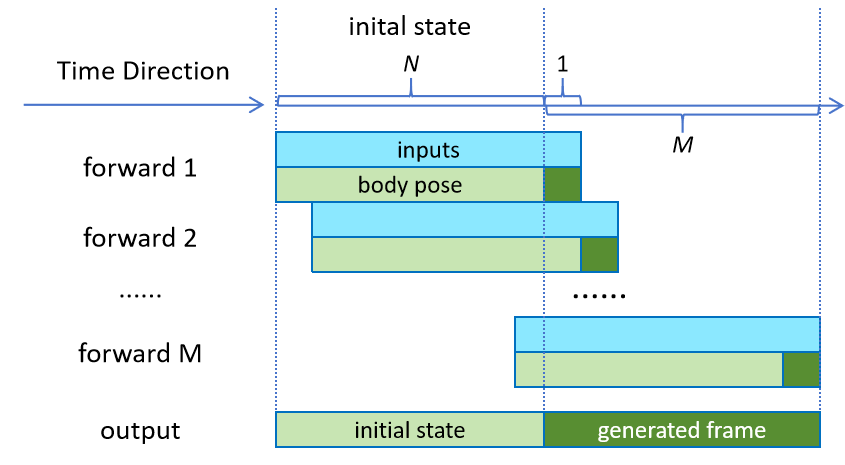
\includegraphics[width=0.75\linewidth]{figures/Fig2.png}
\caption{滑动窗口训练机制:模型通过自回归循环预测 $M$ 帧,每步使用 $N$ 帧上下文并预测第 $N+1$ 帧。损失函数累计所有预测帧的误差,保证因果性与时间平滑性。}
\label{fig2_}
\end{figure}

通过以上适配,FaceCapGes 在保持 CaMN 级联优势的同时显著降低系统延迟,
实现实时稳定的语音与面部驱动手势生成。

然而,仅依赖这两种模态仍存在动作方向与节奏响应不足的问题。
为此,下一节将在级联结构末端引入头部姿态模态,以补充时序反馈与空间方向信号。

\subsection{头部姿态模态的引入与结构位置}

头部姿态在自然交流中是语音与动作之间的重要中介信号,其变化频率高、幅度小,与语音节奏同步显著。与语音和面部不同,头部旋转具备强烈的反应性(reactive)特征:它往往是语义或情感驱动的即时响应,而非主动规划信号。因此,本文将其视为一种“终端模态”(terminal modality),位于级联架构末端,用于补充方向与节奏信息。

\paragraph{输入特征与表示.}
本文仅使用头部旋转信息,不引入平移位移特征。BEAT 数据集中演讲者多为站姿,录制中存在身体移动,若直接使用位移作为输入,噪声易混入;此外,目标应用场景中的坐姿用户分布不同,直接建模位移会削弱泛化性。  
因此仅采用旋转特征,并使用连续且可微的 Rot6d 表示,以避免欧拉角与四元数的奇异性问题。

\paragraph{编码器结构.}
图~\ref{fig_headencoder} 所示为头部姿态编码器结构。该编码器由两层前馈网络组成,输入为 Rot6d 表示的 6 维向量:
\begin{equation}
\mathbf{z}^{H}_t = E_H(\mathbf{H}_{t-N:t}; \mathbf{z}^A_t, \mathbf{z}^F_t),
\end{equation}
其中 $E_H$ 的具体形式为:
\begin{align}
\mathbf{h}_1 &= \mathrm{ReLU}(W_1 \mathbf{H}_t + b_1), \\
\mathbf{z}^{H}_t &= W_2 \mathbf{h}_1 + b_2,
\end{align}
网络维度设置为:输入 $6$,中间层 $36$,输出 $12$。  
在特征层面,其输出与语音、面部嵌入拼接后输入解码器,形成从语义到反应的多层信号流。

\begin{figure}[h!t]
\centering
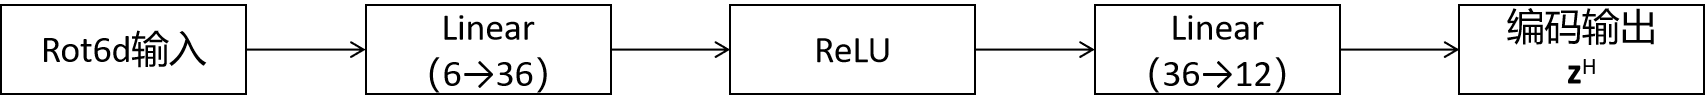
\includegraphics[width=0.8\linewidth]{figures/Fig_headencoder.png}
\caption{头部姿态编码器结构示意图。
输入为 Rot6d 表示的 6 维旋转向量,经两层前馈网络与 ReLU 非线性映射,
输出 12 维紧凑潜在表征。
该编码结果与语音、面部嵌入拼接后输入解码器,用于补充动作的方向与节奏信号。}
\label{fig_headencoder}
\end{figure}

\paragraph{架构位置与实验依据.}
在早期实验中,我们尝试将头部姿态与语音、面部特征早期融合,但该方式导致手势方向轻微抖动、语音与动作节奏错位,收敛速度减慢。分析认为,原因在于头部姿态的反应性与非因果性:若过早参与特征交互,会破坏语音—手势因果映射。  
因此本文采用\textbf{后级融合(late fusion)}策略,在语音与面部特征编码完成后再输入头部特征。该设计使模型先形成语义骨架,再由头部姿态进行方向修正与节奏调节。实验表明,此配置带来更高的自然度与时间对齐性能(见第~\ref{sec:eval} 节)。

\subsection{小结:从语义驱动到反应调节的信号层级}

FaceCapGes 在 CaMN 的语音—表情级联架构基础上,通过实时适配与头部模态引入实现了信号层级的扩展。前两级模态承担语义与情感驱动,而新增头部姿态层作为反应性调节模块,在实时条件下为手势提供动态节奏与空间反馈。

\begin{figure*}[h!t]
\centering
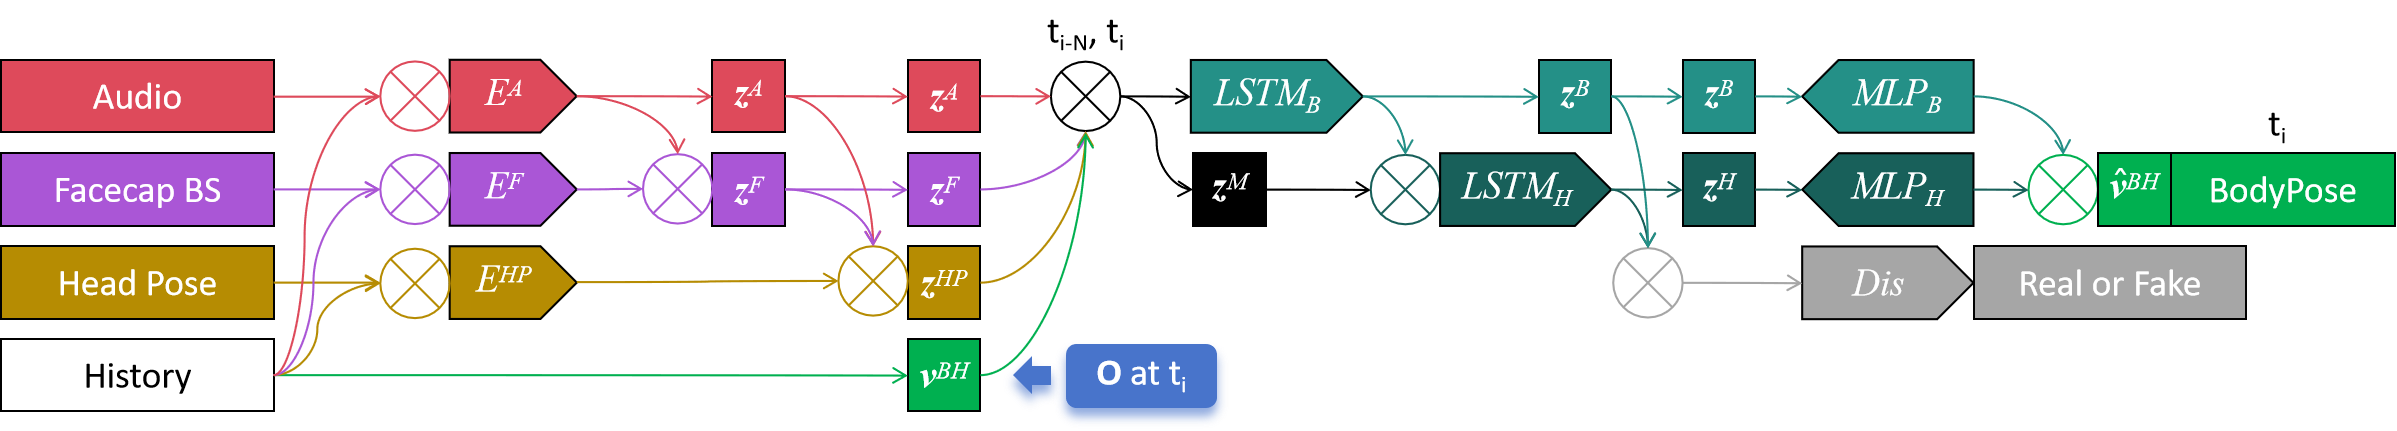
\includegraphics[width=\textwidth]{figures/Fig1.png}
\caption{FaceCapGes 模型结构:音频、面部、头部编码器分别提取模态特征后拼接,输入至 LSTM 解码器生成躯干与手部动作,仅保留最后一帧输出作为当前时刻预测,符合帧级实时推理设定。训练阶段历史姿态序列比目标长度少一帧,需进行零填充。}
\label{fig1_}
\end{figure*}

\section{训练与损失函数设计}

在前述滑动窗口式自回归训练框架下,每段输入序列包含 $N$ 帧上下文与 $M$ 帧预测结果。
模型在每个窗口中输出连续的动作序列 $\hat{\bm{g}} \in \mathbb{R}^{M \times 6 \times 47}$,
并以重构与对抗两类损失共同约束生成质量。

\paragraph{手势重构损失.}
重构项 $\mathcal{L}_{Gesture Rec}$ 由位置、速度与加速度误差组成,用以平衡空间准确性与时间平滑性:
\begin{equation}
\bm{g}' = \bm{g}_t - \bm{g}_{t-1}, \quad \bm{g}'' = \bm{g}'_t - \bm{g}'_{t-1},
\end{equation}
\begin{equation}
\mathcal{L}_{Gesture Rec} = \mathcal{L}_{rec}(\bm{g}, \hat{\bm{g}}) + \mathcal{L}_{vel}(\bm{g}', \hat{\bm{g}}') + \mathcal{L}_{acc}(\bm{g}'', \hat{\bm{g}}''),
\end{equation}
其中 $\mathcal{L}_{rec}$ 保证空间姿态重构精度,
$\mathcal{L}_{vel}$ 和 $\mathcal{L}_{acc}$ 强调动态平滑性与时序一致性。
该组合设计在自回归预测中能有效缓解抖动与速度漂移问题。

\paragraph{对抗损失.}
为进一步提升动作的自然度,引入对抗项 $\mathcal{L}_{Adv}$:
\begin{equation}
\mathcal{L}_{Adv} = -\mathbb{E}[\log(Dis(\hat{\bm{g}}))],
\end{equation}
其中判别器 $Dis$ 以完整的动作序列为输入,
判别其是否来自真实数据分布。
该项损失约束生成序列的整体动力学分布,
促进生成动作在节奏、加速度和能量变化上与真实表演者一致。
训练中通过交替优化生成器与判别器的参数,保持两者的平衡。

\paragraph{总体损失.}
综合两项目标,模型的最终训练目标为:
\begin{equation}
\mathcal{L}_{total} = \mathcal{L}_{Gesture Rec} + \lambda_{adv}\mathcal{L}_{Adv},
\end{equation}
其中 $\lambda_{adv}$ 为对抗损失的权重(实验中设为 $0.1$)。
该设计在保持运动学准确性的同时,提升了时序的自然性与节奏感。

\section{实现与训练配置}

在上述训练目标下,FaceCapGes 基于 PyTorch 实现,
所有实验在单张 NVIDIA RTX 4090 GPU 上进行。

本文基于 BEAT 数据集~\cite{beatcamn} 进行训练与评估。
该数据集包含多模态同步的语音、面部 blendshape 与全身动作信息,
以 15\,fps 记录多位专业表演者的演讲片段,覆盖多种语义与情绪场景。
其标准骨架结构如图~\ref{fig_beatbones} 所示,
共包含 47 个关节节点。
FaceCapGes 仅预测其中的上半身部分,
包括上肢及脊椎的三个主要控制点(蓝色区域所示),
以聚焦语音驱动手势中的表达性动作。
下肢关节保持静态以保证骨架一致性。

\begin{figure}[h!t]
\centering
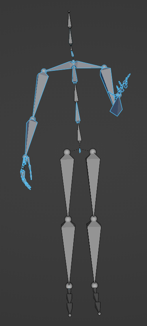
\includegraphics[width=0.15\textwidth]{figures/Fig_BEATBones.png}
\caption{
BEAT 数据集的骨架拓扑结构。
蓝色部分为 FaceCapGes 模型的控制区域,
涵盖上肢与三段脊椎关节,其余节点保持静态。
}
\label{fig_beatbones}
\end{figure}

本文选取表演者 ID~2、4、6、8 的数据进行训练与测试,
其中~2、4~为男性,~6、8~为女性,
确保在性别与说话风格上的分布均衡。
训练集与测试集均包含相同的表演者,
但使用不同的演讲片段,
在预处理阶段已进行严格划分以避免片段交叉。

\paragraph{训练配置.}
训练时输入窗口的前序帧数设为 $N=16$,预测长度为 $M=34$,训练片段的切割步长为 10 帧。
相邻片段因此存在部分重叠,从而在保证充分上下文信息的同时提升数据覆盖率与时间连续性。
优化器采用 Adam~\cite{adam2017},学习率设为 $2\times10^{-4}$,$\beta_1=0.9, \beta_2=0.999$。
批大小设为 256。
为防止早期训练阶段的不稳定,对抗项在第 10 epoch 后引入,整体训练共 374 个 epoch。
在损失计算中,前 $N$ 帧的历史窗口仅作为因果上下文输入,不参与重构与对抗项的误差回传。
损失函数采用第~\ref{sec:loss} 节所述的复合重构与对抗目标。

\paragraph{姿态表示.}
所有身体动作均转换为连续可微的 Rot6d 表示,
使用 EMAGE~\cite{emage} 中的实现方法,
以避免欧拉角奇异性与四元数的符号不确定性。

\paragraph{运行性能.}
在实时推理阶段,FaceCapGes 能以 15\,FPS 的速度驱动虚拟角色,
满足实时语音交互应用的延迟要求。

\section{本章小结}
本章系统介绍了 FaceCapGes 模型的总体设计与关键技术细节。  
首先,从系统整体出发,阐述了实时语音驱动虚拟人生成管线的总体框架,  
说明了模型在输入采集、手势生成与渲染驱动中的定位与功能。
针对基线模型 CaMN 的结构特征,本文在保持多模态级联优势的基础上,  
对时间建模与实时适配机制进行了系统性改进:  
移除了说话人 ID 输入分支,采用独立模型对应不同说话风格;  
引入单向 LSTM 与滑动窗口式自回归训练以保证因果性与流式生成能力。  

在模型的模态设计上,本文重点分析了语音与面部模态的继承机制,  
并在级联架构末端加入头部姿态编码器,以补充方向性与节奏反馈信号。  
同时,结合对抗优化与多级重构损失,构建了兼顾空间准确性与时间自然性的训练目标。  
实验部分将进一步验证这些结构设计对实时性、平滑性与自然度的提升效果。  